% begin module polar-questions
\begin{frame}
\begin{enumerate}
\item<1-| alert@2>  What if $\theta$ is negative?
\item<1-| alert@3>  What if $r$ is negative?
\item<1-| alert@4>  What if $r$ is $0$?
\end{enumerate}
\begin{columns}[c]
\column{.5\textwidth}
\ \uncover<2->{%
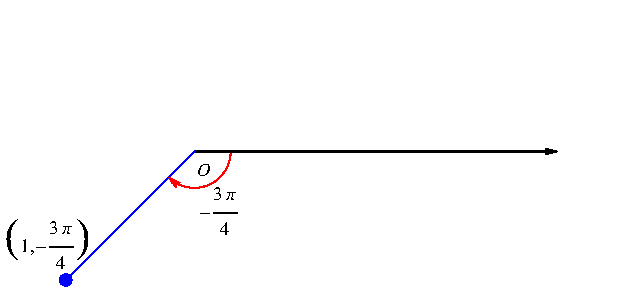
\includegraphics[height=3cm]{polar-curves/pictures/11-03-ex1b.pdf}%
}%
\ \uncover<3->{%
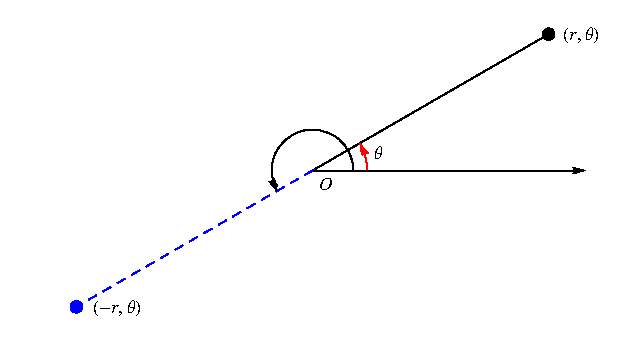
\includegraphics[height=3cm]{polar-curves/pictures/11-03-negativer.pdf}%
}%
\column{.5\textwidth}
\begin{enumerate}
\item<2-| alert@2>  Positive angles $\theta$ are measured in the counterclockwise direction from $O$.  Negative angles are measured in the clockwise direction.
\item<3-| alert@3>  $-r$ and $r$ lie on the same line through $O$ and at the same distance from $O$, but on opposite sides.
\item<4-| alert@4>  If $r = 0$, then $(r, \theta) = P = O$ for all values of $\theta$.
\end{enumerate}
\end{columns}
\end{frame}
% end module polar-questions
